% Generated by analysis/reproduce.py from retained observations.
% Required packages: pgfplots, amsmath, xcolor, tikz
% Required TikZ libraries: none
% Target width: 160 mm maximum, use at natural size
% Minimum text size: 8.5 pt
% Colour/greyscale intent: one teal accent; shape and dash cues survive greyscale
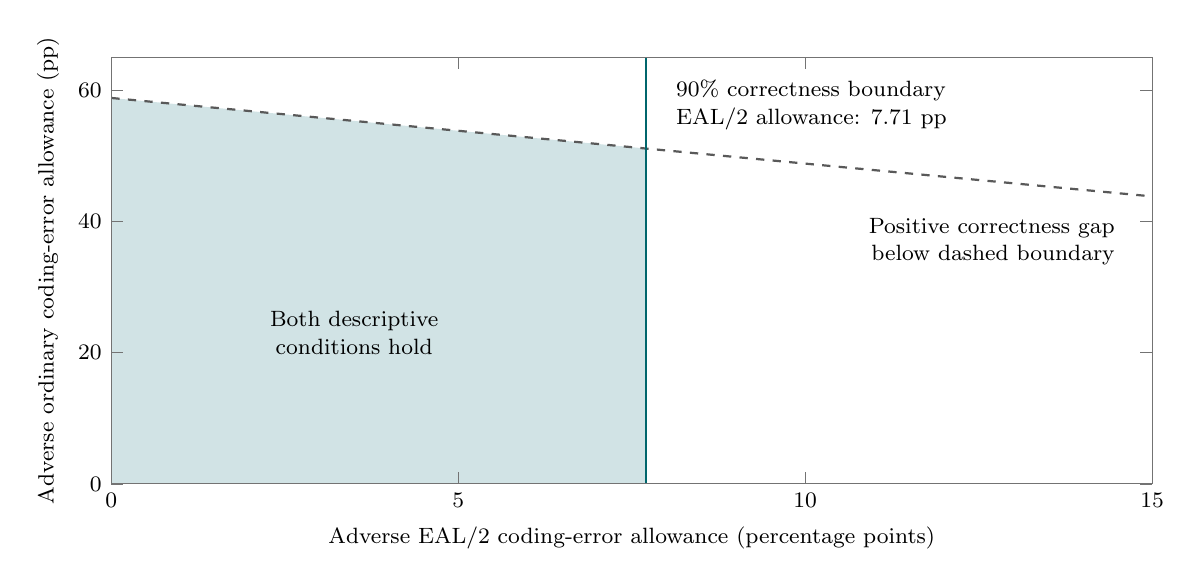
\begin{tikzpicture}
\definecolor{ealteal}{RGB}{0,102,108}
\pgfplotsset{compat=1.18,ealaxis/.style={font=\fontsize{8.5}{10}\selectfont,
  tick label style={font=\fontsize{8.5}{10}\selectfont},
  axis line style={black!55,line width=0.4pt},tick style={black!55},
  grid style={black!12,line width=0.35pt},axis on top,
  legend style={draw=none,fill=white,font=\fontsize{8.5}{10}\selectfont},legend cell align=left,
  label style={font=\fontsize{8.5}{10}\selectfont}}}
\begin{axis}[ealaxis,width=14.8cm,height=7cm,xmin=0,xmax=15,ymin=0,ymax=65,xtick={0,5,10,15},ytick={0,20,40,60},
xlabel={Adverse EAL/2 coding-error allowance (percentage points)},ylabel={Adverse ordinary coding-error allowance (pp)}]
\addplot[draw=none,fill=ealteal!18] coordinates {(0.00000000,0.00000000) (7.70833333,0.00000000) (7.70833333,51.09375000) (0.00000000,58.80208333)} \closedcycle;
\addplot[black!65,dashed,line width=.8pt] coordinates {(0.00000000,58.80208333) (15.00000000,43.80208333)};
\addplot[ealteal,line width=.9pt] coordinates {(7.70833333,0.00000000) (7.70833333,65.00000000)};
\node[align=center,font=\fontsize{8.5}{10}\selectfont] at (axis cs:3.5,23) {Both descriptive\\conditions hold};
\node[anchor=north west,align=left,font=\fontsize{8.5}{10}\selectfont] at (axis cs:8.0,63) {90\% correctness boundary\\EAL/2 allowance: 7.71 pp};
\node[anchor=north east,align=right,font=\fontsize{8.5}{10}\selectfont] at (axis cs:14.6,42) {Positive correctness gap\\below dashed boundary};
\end{axis}
\end{tikzpicture}
